\documentclass[english,a4paper,twoside]{report}

% Used packages
\usepackage[printonlyused]{acronym}
\usepackage{amsfonts}
\usepackage{amsmath}
\usepackage{amssymb}
\usepackage{babel}
\usepackage{calc}
\usepackage{fancyhdr}
\usepackage{graphicx}
\usepackage{listings}
\usepackage{url}

\newcommand{\Rvk}{Reykjav\'\i{}k }
\newcommand{\AmbE}{Ambient~Earth}
\newcommand{\Amber}{Amber}

% Global settings.
\setlength{\parskip}{\medskipamount}
\setlength{\parindent}{0pt}

% Listing settings.
\lstset{basicstyle=\fontfamily{cmss}\small,frame=tb}
\lstset{columns=fixed,basewidth=0.5em,keepspaces=true}
\lstset{aboveskip=1em,belowskip=0.5em}
\lstset{numbers=left,numberstyle=\tiny,stepnumber=5}
\lstset{showtabs=false,showspaces=false,showstringspaces=false}

% Improved title page.
\makeatletter
\newcommand{\institution}{\newcommand{\@institution}}
\renewcommand\maketitle{\begin{titlepage}%
\let\footnotesize\small
\let\footnoterule\relax
\let \footnote \thanks
\null\vfil
\vskip 60\p@
\begin{center}%
  {\LARGE \@title \par}%
  \vskip 3em%
  {\large
   \lineskip .75em%
    \begin{tabular}[t]{c}%
      \@author
    \end{tabular}\par}%
    \vskip 1.5em%
  {\large \@date \par}%       % Set date in \large size.
\end{center}\par
\@thanks
\vfill
{\small
 \begin{flushright}
  \begin{tabular}{l}\hline
  \@institution\hline
  \end{tabular}
 \end{flushright}
}
\global\let\@institution\@empty
\global\let\institution\relax
\end{titlepage}
}

% Improved acronym environment.
\newenvironment{acronym*}[1]{%
   \newcommand{\acrolabel}[1]{\textbf{##1}\hfil}%
   \providecommand*{\acro}{\AC@acro}%
   \begin{list}{}{%
      \renewcommand{\makelabel}{\acrolabel}%
      \settowidth{\labelwidth}{\textbf{#1}}%
      \setlength{\leftmargin}{\labelwidth+\labelsep}%
      }
   }{%
   \end{list}
}\makeatother

% Fancy header settings.
\pagestyle{fancy}
\renewcommand{\chaptermark}[1]{\markboth{#1}{}}
\renewcommand{\sectionmark}[1]{\markright{\thesection\ #1}}
\fancyhf{}
\fancyheadoffset[LE,RO]{\marginparsep+\marginparwidth}
\fancyhead[LE,RO]{\bfseries\thepage}
\fancyhead[LO]{\bfseries\rightmark}
\fancyhead[RE]{\bfseries\leftmark}
\fancypagestyle{plain}{%
  \fancyhead{}\renewcommand{\headrulewidth}{0pt}}

% Document meta data.
%FIXME: better title & remove draft suffix
\title{Ambient Earth\\
       {\Large \emph{Design Document --- 1$^{\text{st}}$ draft\/}}}
\author{Christian Luijten\\\url{christian06@ru.is}}
\date{\today}
\institution{
 CADIA group \\
 School of Science and Engineering \\
 \Rvk University, \Rvk \\[1em]
 \emph{Under supervision of:\/} \\
 Kristinn R. Th\'orisson, Ph.D. (\Rvk University) \\
 dr.ir. Huub van de Wetering (Eindhoven University of Technology) \\
}

% Macros.
\newcommand{\anode}[1]{\textsl{#1\/}}
\newcommand{\atype}[1]{\ensuremath{\textsl{#1\/}}}
\newcommand{\content}[1]{\textsl{#1\/}}
\newcommand{\entry}[1]{\texttt{#1}}
\renewcommand{\implies}{\Rightarrow}
\newcommand{\pole}{\addtocounter{fd@flagcount}{1}}
\newcommand{\mblstinline}[1]{\mbox{[\lstinline[columns=fixed]{#1}]}}
\newcommand{\q}{\quad}
\newcommand{\strtok}[1]{\textbf{`#1'}}

\begin{document}

\acrodef{RU}{\Rvk University}
\acrodef{CADIA}{Center for Analysis \& Design of Intelligent Agents}

\maketitle

\abstract{
  Ambient Earth is...
 }

\tableofcontents

\chapter{Introduction}

This document describes the design of the \AmbE\ project. The ambitional goal
of this project is to give an ambient view on the activity on the whole
world-wide web. In practice, it shows the activity on for instance a forum or
larger weblog system.

The design of the project will follow the Constructionist Design
Methodology for Interactive Intelligences\cite{CDM}.


\chapter{Usage scenarios}

\section{A story is posted to a weblog}

When a story is posted on a weblog, it will show up in its RSS feed (this
happens of course outside of our responsibility). If \Amber\ is monitoring this
particular weblog, it will retrieve the story and analyze it. The story is then
displayed on a screen using the results of the analysis.

To get a more concrete idea, suppose \Amber\ is monitoring various A.I. related
weblogs and we would like to find out what they are mainly writing about. We
configure the analysis component in such a way that it can decide whether a
certain subject is dealt with in a story, thereby creating a profile for every
story. Stories with similar subjects will then show up close to eachother in
the display, stories with orthogonal subjects will be very far apart.

The result is an image with various ``clouds'' of in some way related stories.

\section{A discussion is held on a web forum}

Discussions on web forums can get lengthy and the main subject can change
multiple times during their lives. To get an idea what subjects the whole
discussion has been about, \Amber\ can show a cloud map of (part of) the
discussion. It could even show an animation to show how the discussion
developed over time.


\chapter{\label{cpt:requirements}Requirements}

There are various kinds of requirements to be identified. A distinction can be
made between functional and extra-functional (or non-functional) requirements.

\section{Extra-functional requirements}

\begin{enumerate}
  \item The system must make use of the Psyclone framework for communication.
  \item The system will be implemented in the Java programming language.
  \item The display module with the Java Applet must be able to run on any
        machine with a properly installed Java Virtual Machine (i.e. not only
        on the machine running the rest of the system).
  \item It must be possible to add modules with similar functionality to
        operate in parallel with modules already there. For example when the
        Java Applet is running, it should also be possible to have the full
        screen module running at the same time. 
\end{enumerate}

\section{Functional requirements}

These requirements describe which \emph{inputs}, \emph{outputs}, \emph{storage}
and \emph{computations} exist in the system and how they are \emph{timed and
synchronized}. Finally, since this is a very important part of the project,
there are two separate sections on \emph{story analysis} and
\emph{visualization} requirements.

\subsection{Inputs}

\begin{enumerate}
  \item The system must be configurable to specify which sources will be
        monitored.
  \item The system will use the configuration to get information from the
        internet from the specified sources.
  \item Configuration of the system goes via Psyclone using module parameters.
  \item The display may have a set of controls to navigate through the history
        of a feed.
  \item Parts of the system must accept triggers from Psyclone whiteboards.
  \item Sources must be \ac{RSS} feeds. The system should however be prepared
        to support other source types as well (i.e. it should be easily
        expandable).
  \item The Applet display is non-interactive (no input).
\end{enumerate}

\subsection{Outputs}

\begin{enumerate}
  \item There is an output module which is to be used within a website,
        i.e. a Java Applet.
  \item There is an output module which runs standalone and in full screen
        and displays more information than the Applet can.
\end{enumerate}

\subsection{Storage}

\begin{enumerate}
  \item The system on itself does not store anything.
\end{enumerate}

\subsection{Computations}

\begin{enumerate}
  \item The system must decide of a delivered story what its subject(s) is/are.
  \item The system may put weights on the subjects instead of a boolean value.
\end{enumerate}

\subsection{Timing and synchronization}

Synchronization between modules is handled by Psyclone, so no requirements need
to be added to the system itself.

\subsection{Story analysis}

\begin{enumerate}
  \item When stories come in, they are analysed by analysis modules.
  \item Every module adds some meta-information to the story depending on the
        module analysis.
\end{enumerate}

\subsection{Visualization}

The following requirements are common for both the applet and the standalone
viewer.

\begin{enumerate}
  \item A story is represented as a dot.
  \item In the center of the display is Earth (with picture?).
  \item Dots are launched into orbit around Earth.
  \item The orbits follow Kepler's laws of planetary motion.
  \item The launch velocity is dependent on how ``big'' the story is (like from
        an important author or if it has many references) at the time of
        writing, but is always smaller than the escape velocity.
  \item Stories get velocity boosts by getting replies/comments or
        references (``trackbacks'') in order to keep them around longer.
  \item Stories which don't get reactions will just orbit Earth for a while and
        eventually fall back down \mbox{(i.e. launch velocity $<$ escape
        velocity)}.
  \item Only the meta-information added to the stories by the Sieve modules is
        used to determine launch variables.
  \item There are some small, heavy bodies in geostationary orbit around Earth
        representing values of an enumeration of meta-information (for instance
        story subjects). They attract the stories depending on how much they
        match the story's subject. It is possible for a story to get into orbit
        with such a heavy body if it is really strongly connected to the
        subject.
\end{enumerate}

There will be two different views, a static and a dynamic one. Which one is
used depends on the application. To get an idea of the activity at a certain
moment in time, the static view is used. For a ``real-time'' view of internet
activity, the dynamic view can be used.

The term ``static'' doesn't mean the image is standing still, it will behave
exactly the same as the dynamic view. However, some physical laws don't apply
or are differently calibrated in order to give a constant image. In other
words, while in dynamic view stories can appear and disappear, in the static
view the stories are a given constant.

\subsubsection{Differences between Applet and Standalone viewer}

\begin{enumerate}
  \item The applet display will in practice be considerably smaller than the
        standalone viewer. Therefore, the applet is less detailed and some
        physical laws might need to be bend a bit.
\end{enumerate}



\chapter{\label{cpt:architecture}Architecture}

The architecture of \Amber\ is defined in terms of modules and the messages
they use to communicate. A global architecture is depicted in
Figure~\ref{fig:global-architecture}.

In the Section~\ref{sct:modules} the modules are described in detail and in
Section~\ref{sct:messages} the messages connecting the modules are defined.

\begin{figure}
    \centering
    \frame{Here be pretty and good images}
    \caption{\label{fig:global-architecture}Global \Amber\ architecture}
\end{figure}

\section{\label{sct:modules}Modules}

A complete Amber system will comprise at least three modules running at the
same time; there is a Crawler module, a selector module called Sieve and a
display called ShowOff. The modules are separate executables with their own
life-cycles and resources.

Every module has a specified interface through which communication with
Psyclone is handled.

\subsection{Crawler modules}

\begin{figure}
    \centering
    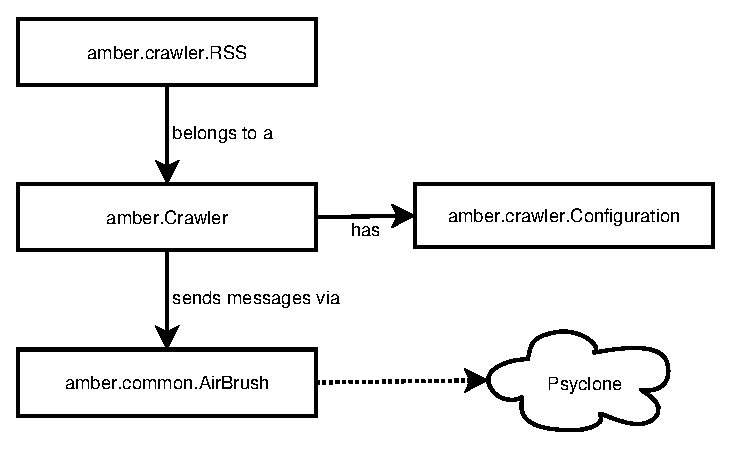
\includegraphics{image/crawler}
    \caption{Diagram of the design of the Crawler, the names are Java classnames}
\end{figure}

When the Crawler is started, it will create one of the available handlers
(depending on what is specified on the command line or what is set as default
during build time). 

It also creates an AirBrush instance to communicate with Psyclone via
Java\-Open\-AIR. The module name announced to Psyclone is `Crawler.' plus the
name of the handler, so `Crawler.RSS' in case of the RSS handler.

After connecting with Psyclone, the handler can get its parameters stored in
the psySpec file and go to work. It will post stories with type
`External.Crawler.$\langle$handler$\rangle$.Story' (i.e.
`External.Crawler.RSS.Story') on the whiteboard `WB.Stories.Raw'.

\subsubsection{RSS}

The RSS crawler module will be fairly straightforward. There are actually quite
a few good RSS parsers around for Java, the only thing the crawler should do is
getting the stories from the RSS feeds along with meta-information and store it
on the whiteboard.

\begin{module}{amber.crawler.RSS}{Crawler.RSS}
    \post{External.Crawler.RSS.Story}{WB.Stories.Raw}{A story}
\end{module}

\subsubsection{DiggAPI}

Digg is a website which lets users submit stories found on the web. Other users
then moderate the submissions either by `digging' or `burying' a story. A story
with a lot of `diggs' is a popular one. The nice thing about Digg is that it
actually does a lot of work for the \Amber\ system.

Digg
announced\footnote{\url{http://diggtheblog.blogspot.com/2006/07/digg-labs-launches-alpha.html}}
that they will publish a public API within the next months. If time allows, a
DiggAPI module is created.

\begin{module}{amber.crawler.DiggAPI}{Crawler.DiggAPI}
\end{module}

% \subsubsection{BloggerDataAPI}
% 
% One of the larger weblog hosters is Google with their Blogger service. There
% is an API available to get information from it.

\subsection{Sieve modules}

Every invocation of a Sieve on a Story will decrease its \texttt{processLeft}
value until it is 0. When it reaches 0, the story is moved to the ``processed''
whiteboard WB.Stories.Processed.

\subsubsection{KeywordSpotter}

The KeywordSpotter is configured to detect the presence of certain keywords in
a story which makes it fit in a certain category or subject. In early versions
the weights of the subjects will be equal. In later versions all weights of all
subjects of a story must for instance add up to 100\%. This gives the
visualizer more freedom to place the story.

\begin{module}{amber.sieve.KeywordSpotter}{Sieve.KeywordSpotter}
    \post{Internal.*}{WB.Stories.Processed}{Thingy}
    \trigger{External.Crawler.*.Story}{WB.Stories.Raw}{Thingy}
\end{module}

\subsubsection{PhraseSpotter}

The PhraseSpotter will use a grammar engine to detect whether certain types of
sentences appear in a story to classify it.

\begin{module}{amber.sieve.PhraseSpotter}{Sieve.PhraseSpotter}
\end{module}

\subsection{ShowOff modules}

\begin{figure}
    \centering
    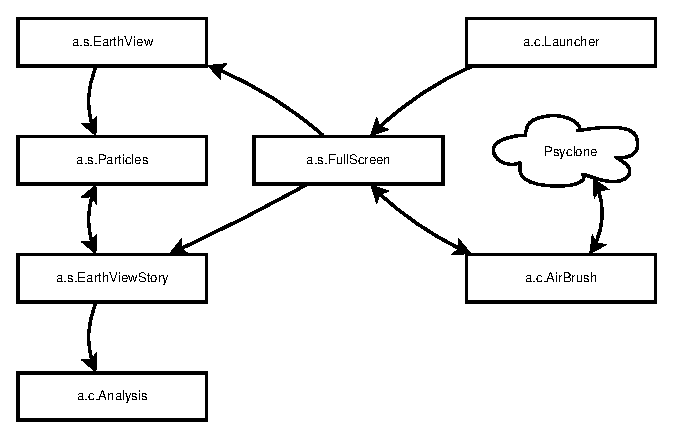
\includegraphics{image/showoff-fullscreen}
    \caption{Diagram of the design of the full screen ShowOff module, the names are abbreviated Java classnames}
\end{figure}

\subsubsection{Full screen}

The full screen application will display a lot of information and is there to
be looked - not glanced - at. It should be possible to let it do its job
autonomously, just showing a pretty picture, or to be interactive.

\begin{module}{amber.showoff.FullScreen}{ShowOff.FullScreen}
\end{module}

\subsubsection{Ambient applet}

The ambient applet will display a very easy to understand image of the status
of the page it is on. I.e. if the page is a weblog, it should display subject
information on that weblog, if it is on the page of a thread of a forum, it
displays the flow of the discussion.

\begin{module}{amber.showoff.Applet}{ShowOff.Applet}
\end{module}



\section{\label{sct:messages}Messages}


\subsection{Between Crawler and Sieve}


\subsection{Between Sieve and ShowOff}






\chapter{Conclusion}


% \appendix

\bibliographystyle{cadia}
\bibliography{bibliography}
\addcontentsline{toc}{chapter}{\refname}

\end{document}
